\documentclass[12pt]{article}
\usepackage{indentfirst}
\usepackage{siunitx}
\usepackage{graphicx}
\usepackage{subfigure}
\usepackage{float}
\usepackage{subcaption}

\setlength{\parindent}{20pt}
\setlength{\oddsidemargin}{0.5cm}
\setlength{\evensidemargin}{0.5cm}
\setlength{\marginparsep}{0.75cm}
\setlength{\marginparwidth}{2.5cm}
\setlength{\textwidth}{150mm}
\renewcommand{\baselinestretch}{1.5}

\begin{document}
	\begin{titlepage}
		\vspace*{\stretch{1.0}}
		\begin{center}
			\Large\textbf{Report of Resonance Air Column}\\
			\Large\textmd{WU, Chenhao}\\
			\Large\textmd{Student ID: 117010285}\\
			\Large\textmd{November 23rd, 2018}\\
		\end{center}
		\vspace*{\stretch{2.0}}
	\end{titlepage}

	\section{Introduction}
	In this experiment, we tried to investigate the relationship between the length of the tube and the frequencies at which resonance occurs by using a mini speaker, a air column, a piston and a voice sensor. Since that when resonances occur in the air column the voice sensor would receive the maximum amplitude of the sound wave, the experimental frequencies were recorded, which has the maximum amplitude while the position of piston being adjusted in order to construct different length of air column.\par 
	The objective of the experiment is to investigate the relationship and to show that the experimental results are approximately the same to the theoretical results.
	
	\section{Theory}
	When the diaphragm of a speaker vibrates, a sound wave is produced that propagates through the air. The sound wave consists of small motions of the air molecules toward and away from the speaker. General speaking, a sound wave propagates out in all directions from the source of the wave. However, the study of sound waves can be simplified by restricting the motion of propagation to one dimension, as is done with the Resonance Air Column. \par
    In physics, sound wave is a vibration that typically propagates as an audible wave of pressure, through a transmission media such as a gas, liquid or solid. It can be reflected from some places and return waves can interfere the original wave. In the experiment, the sound wave can be reflected many times back and forth between the ends of the fube and all the reflections will interfere together. Under this condition, if the sound wave is of certain frequencies, the reflected waves will be in phase, leading to a very high amplitude standing wave (the sound in the tube is loudest). Such a phenomenon is called resonance and the special waves are call standing waves. \par
    Similar to the nodes and antinodes of a standing wave on a string, a standing wave in the air has: displacement nodes, where the air's vibration is small, and the displacement antinodes, where the amplitude of the air vibration gains its maximum; pressure nodes and pressure antinodes where the air pressure gains its maximum and minimum, corresponding to the displacement antinodes and displacement nodes respectively. \par
    For an open close tube, when resonance occurs there will be a node and an antinode at each end of the tube. According to the number of the nodes, we can define the first resonance, the second resonance, and so on. For an open tube, there will be two antinodes at the two ends of the tube. Similarly, we can define the fundamental resonance, the first resonance, the second resonance, and so on. \par
    When resonance occurs, the length of the tube $L$ and the frequencies of the sound wave $\lambda$ have the following relationship\\
    For Closed Tube
    \begin{equation}
        L = \frac{n\lambda}{4},\, n = 1, 3, 5, 7, 9, ...
    \end{equation}
    where L is the length of the air column. \\
    For Open Tube
    \begin{equation}
        L = \frac{n\lambda}{2},\, n = 1, 2, 3, 4, 5, ...
    \end{equation}
    where L is the tube length. \par
    However, in the reality the effective length of the tube is slightly longer than the measured len gth. Ther approximate description of the resonance requirements for standing waves is given by the following empirical formulas\\
    For Closed Tube
    \begin{equation}
        L+0.3d = \frac{n\lambda}{4},\, n = 1, 3, 5, 7, ...
    \end{equation}
    For Open Tube
    \begin{equation}
        L + 0.6d = \frac{n\lambda}{2},\, n = 1, 2, 3, 4, ...
    \end{equation}
    where d is the diameter of the tube.
    \subsection{Theory of Experiment 1}
    A resonating air column in a tube with one end open and the other end closed will have a node at the closed end and a anti-node at the open end. A node represents an area where the displacement of the air is minimum, and an anti-node represents an area where the displacement of the air is maximum. If the air column in resonating in the fundamental mode (lowest possible frequency) it will have no other nodes or anti-nodes This is shown in Figure 1. \par
    \begin{figure}[H]
    	\centering
    	\subfigure{}{
    		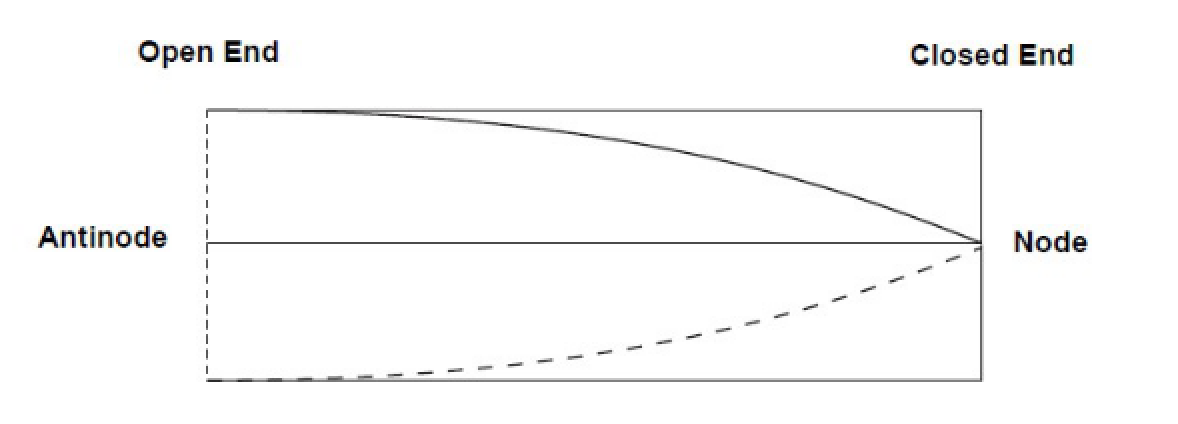
\includegraphics[width=\textwidth]{/home/vitowu/Documents/CourseMaterials/CourseMaterials/PHY1002-Physics_Laboratory/e7/Figure1.png}
    	}
    	\caption{One end open and the other closed}
    \end{figure}
    
    On a sine wave, the distance from one of the maxima to the next point where it crosses zero is a quarter wavelength. Thus, for an air column in a tube with one open end and one closed end, the length of the resonating air column, $L$, and the wavelength, $\lambda$ are related by
    \begin{equation}
        \lambda = 4L
    \end{equation}
    For all types of waves, the relationship between the frequency $f$ and the velocity $v$ of the wave is 
    \begin{equation}
    	v = f \lambda
    \end{equation}
    For a resonating air column in a tube, $v$ is the speed at which sound travels through the air, and $f$ is the frequency of the sound which is the frequency of the Sine Wave Generator in this experiment. \par
    Combining equation (5) and equation (6) yields
    \begin{equation}
    	L = \frac{v}{4f}
    \end{equation} 
 	The length of the air column is inversely proportional to the fundamental frequency.
 	\subsection{Theory of Experiment 2}
 	A resonating tube with both ends open will always have an anti-node at another end, and at least one node in between. The number of nodes is related the wavelength and the harmonic. As shown in Figure 2, the first harmonic has one node, the second harmonic has two, etc.
 	\begin{figure}[H]
 		\centering
 		\subfigure{}{
 			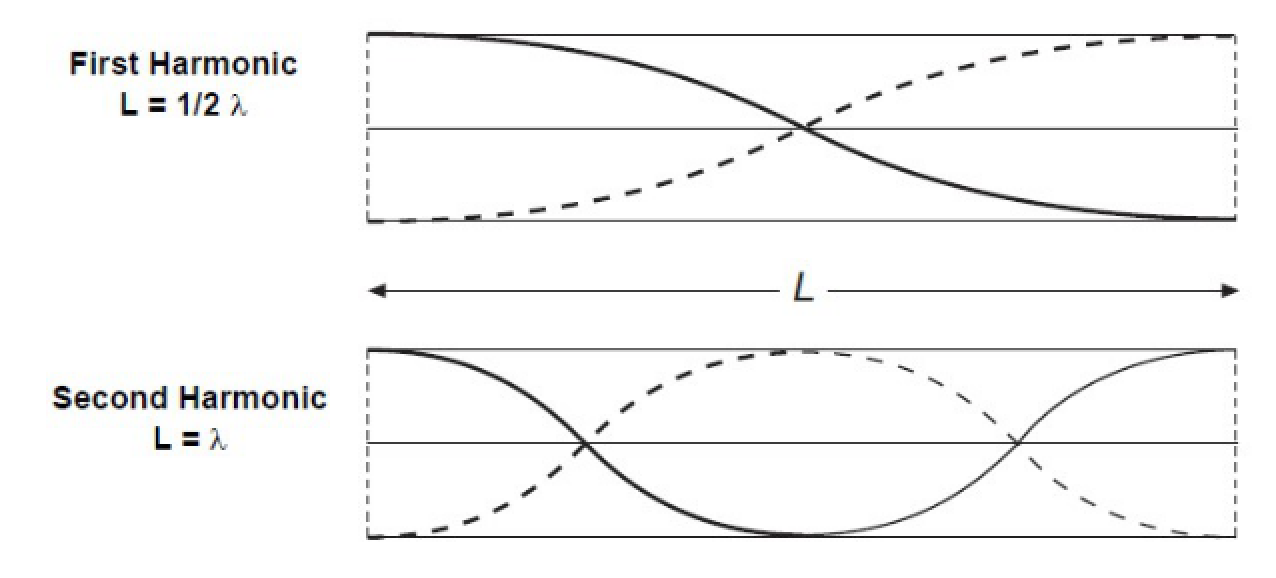
\includegraphics[width=\textwidth]{/home/vitowu/Documents/CourseMaterials/CourseMaterials/PHY1002-Physics_Laboratory/e7/Figure2.png}
 		}
 		\caption{Figure 1. Both ends open}
 	\end{figure}
 	At higher harmonics, the frequency is higher and the wavelength is shorter. Similarly for the fundamental resonance of an open tube, we have
 	\begin{equation}
 		\lambda = 2L
 	\end{equation}
 	\begin{equation}
 		L = \frac{v}{2f}
 	\end{equation}
 	
 	\section{Experiment Procedures}
 	\subsection{Setup}
 	\subsubsection{Quantities Measurements and Constance}
 	Before the experiment, we need to measure some quantities of the instruments,
 	\begin{itemize}
 		\item The length of the air column in the cube: $ L $;
 		\item The diameter of the tube: $ d_{tube} $;
 	\end{itemize}
 	\subsubsection{Equipments}
 	The equipments and the respective model we used in the experiment are listed as following,
 	\begin{itemize}
 		\item Resonance Air Column, 120 cm
 		\item Adjustable Foot
 		\item Piston and Handle
 		\item Marker Clip
 		\item Mini Speaker, Model No.WA-9605
 		\item Signal Generator 
 		\item 550 Universal Interface, Model No.UI-5001
 		\item Banana Plug Patch Cords
 	\end{itemize}
 	\subsubsection{Pre-Installation}
 	1. Package the Resonance Air Column and the adjustable feet such that each adjustable foot is about 2cm away from the end of the tube. \par 
 	2. Put the Mini Speaker at the end of the tube and such that its face towards the cube. \par 
 	3. Set the frequency of the signal generator to 100Hz and the amplitude to zero. Turn on the signal generator. Slowly adjust the amplitude of the signal until a sound from the speaker can be heard.
 	\subsubsection{Installation of Experiment 1}
 	1. Insert the piston into the tube at the end opposite to the Mini Speaker. \par
 	2. Use Spare Marker Clips to record the positions of the piston which make resonance. 
 	\subsubsection{Installation of Experiment 2}
 	1. Keep the position of instruments as Experiment 1. \par 
 	2. Remove the piston since that piston will not be used in Experiment 2.
 	\subsection{Experiment}
 	\subsubsection{Experiment 1}
 	1. Put piston into the tube such that its end is 110 cm from the other end of the tube. \par 
 	2. Set the Signal Generator starting from 50 Hz and increase the amplitude of the generator to a proper level so that the speaker can be heard.\par 
 	3. Slowly increase the frequency of the signal generator and put the acoustic sensor at the closed end of air column near the mini speaker to detect the resonance. The loudness of the sound will increase noticeably when the frequency is within a few hertz of the fundamental frequency. Let the signal generator generate the signal under sweep type to adjust the frequency up from 50 Hz to 100 Hz. \par
 	4. Observe the graph on PASCO to determine at what frequency the sound is loudest and record the experimental results in a table. \par
 	Take data at 10 cm intervals down to a length of 40 cm, repeat step 1-4 for each length.
 	\subsubsection{Experiment 2}
 	1. Turn on the mini speaker and start with the frequency at 50 Hz. \par 
 	2. Slowly increase the frequency of the speaker, and observe the graph on PASCO to find out at what frequency the sound is the loudest. Find and record the frequency of the fundamental by listening for resonance.\par 
 	
 	\section{Experimental Data}
 	\subsection{Error Estimation}
 	The data we measured is include: the length of the air column measured by a ruler, the diameter of the tube measured by the vernier scale and the frequency of the mini speaker.
 	\begin{itemize}
 		\item $ L $: the estimated error of a common ruler is $\SI{\pm0.05}{\centi\meter}$;
 		\item $ d_{tube} $: the estimated error of a vernier scale is calculated by $ \pm0.5\times resolution $, which is $ \SI{\pm0.0005}{m\meter} $;
 		\item Frequency: according to the manual, the resolution of frequency is 0.001Hz.  estimated 
 	\end{itemize}
 	
 	\subsection{Raw Data}
 	\subsubsection{Experiment 1}
 	\begin{figure}[H]
 		\centering
 		\subfigure{}{
 			\centering
 			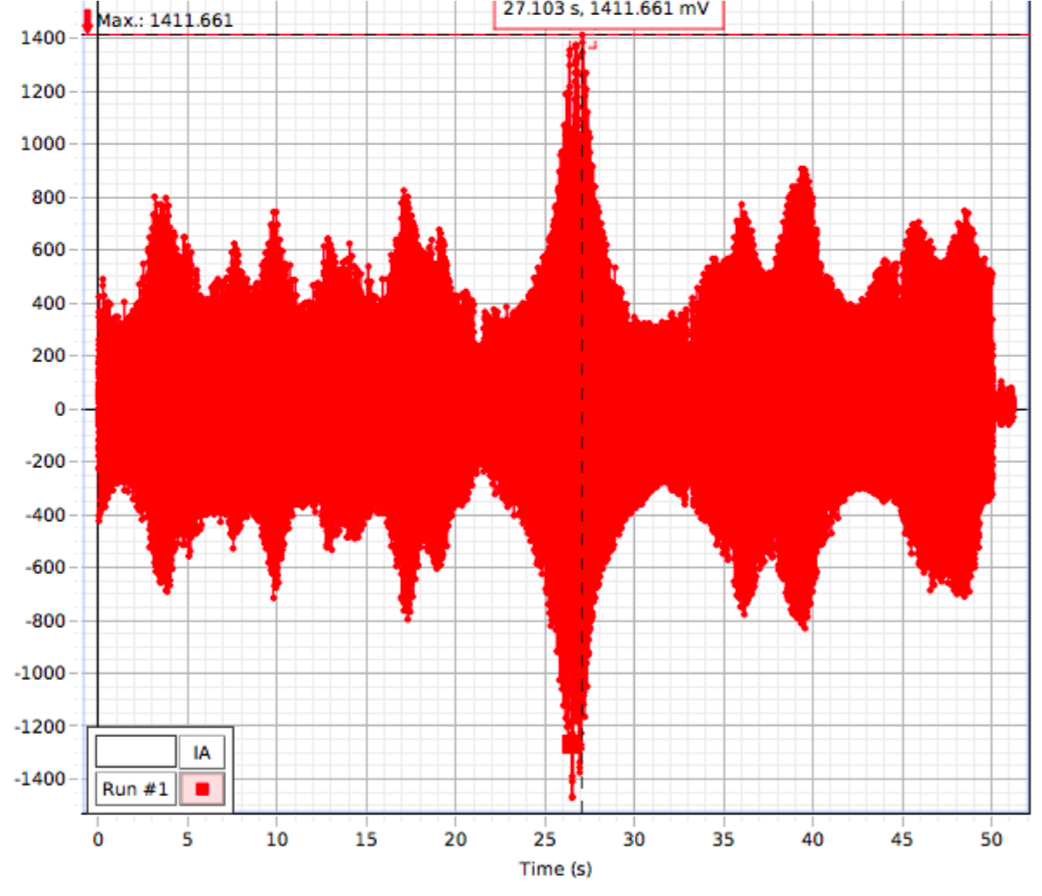
\includegraphics[width=.45\linewidth]{/home/vitowu/Documents/CourseMaterials/CourseMaterials/PHY1002-Physics_Laboratory/e7/110cm.png}
 			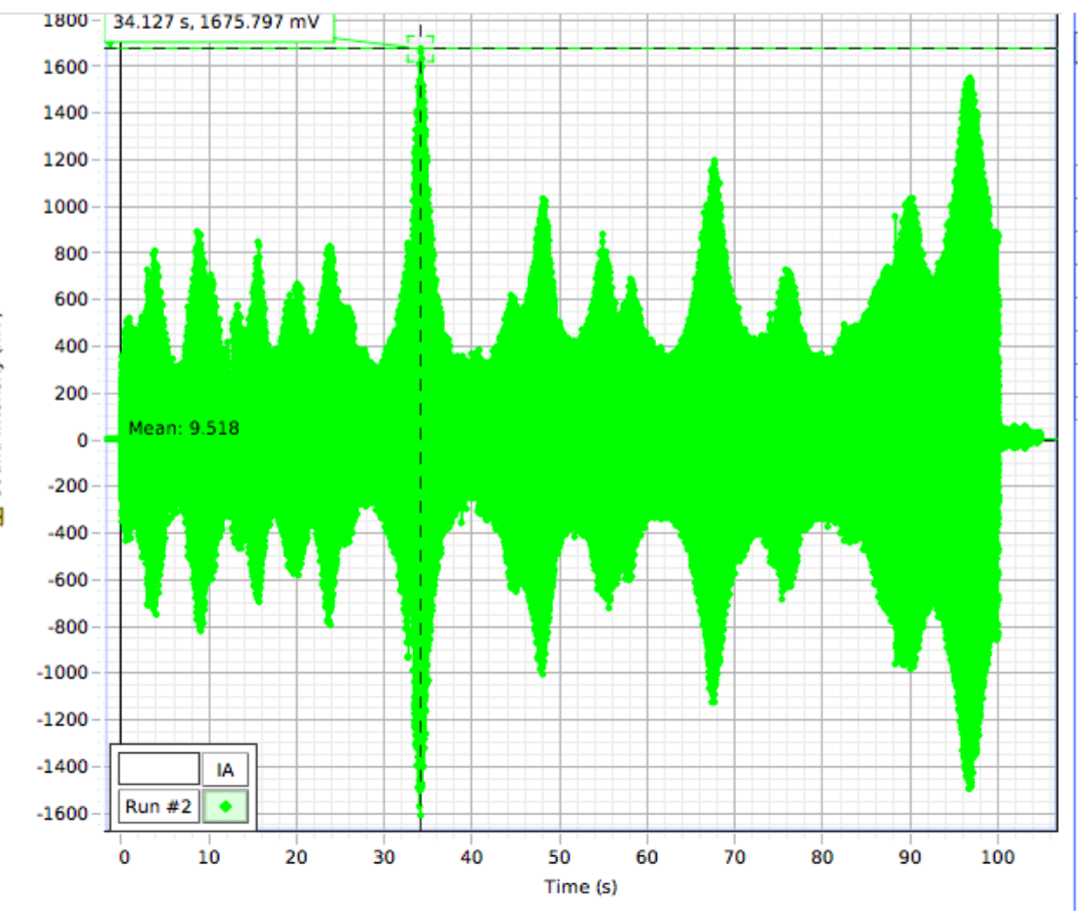
\includegraphics[width=.45\linewidth]{/home/vitowu/Documents/CourseMaterials/CourseMaterials/PHY1002-Physics_Laboratory/e7/100cm.png}
 		}
	 	\subfigure{}{
	 		\centering
	 		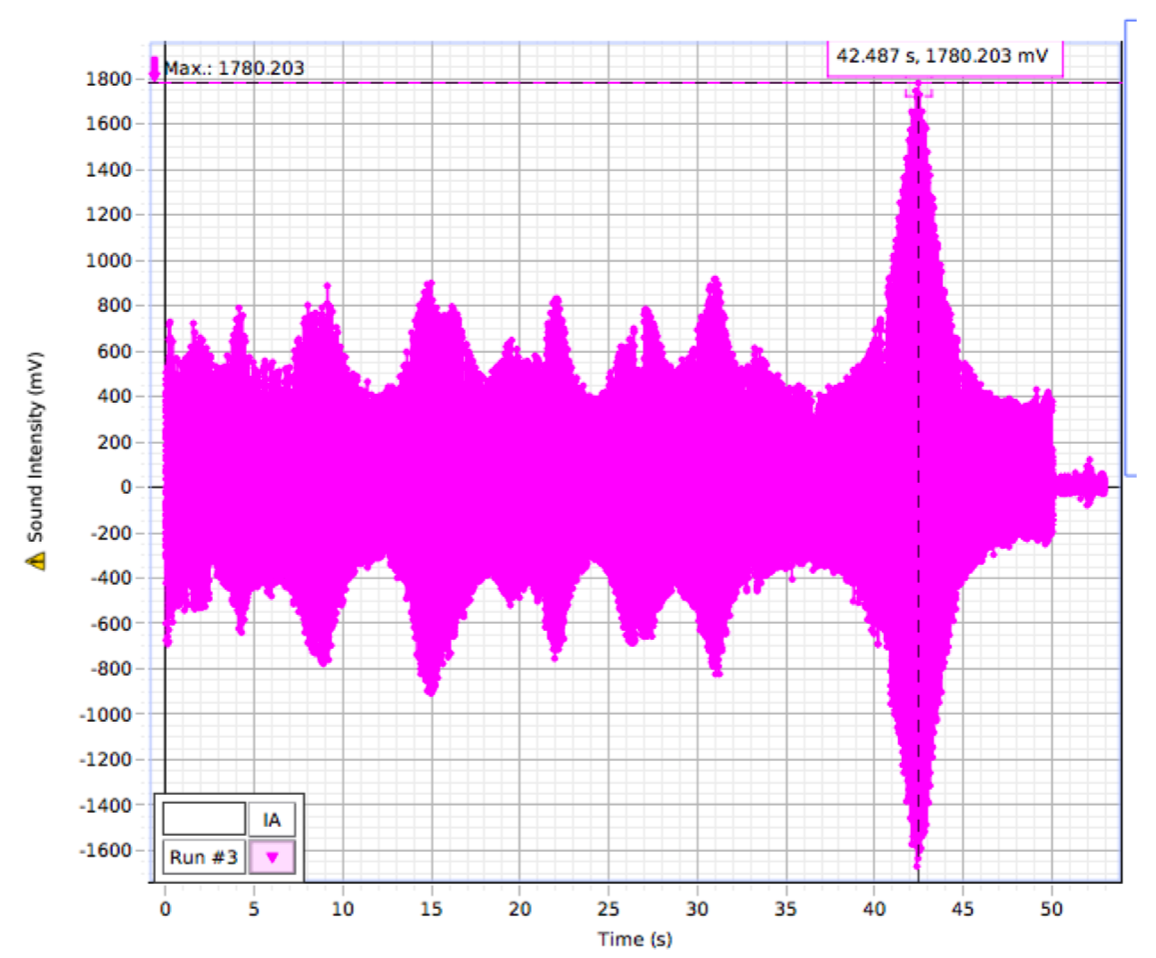
\includegraphics[width=.45\linewidth]{/home/vitowu/Documents/CourseMaterials/CourseMaterials/PHY1002-Physics_Laboratory/e7/90cm.png}
	 		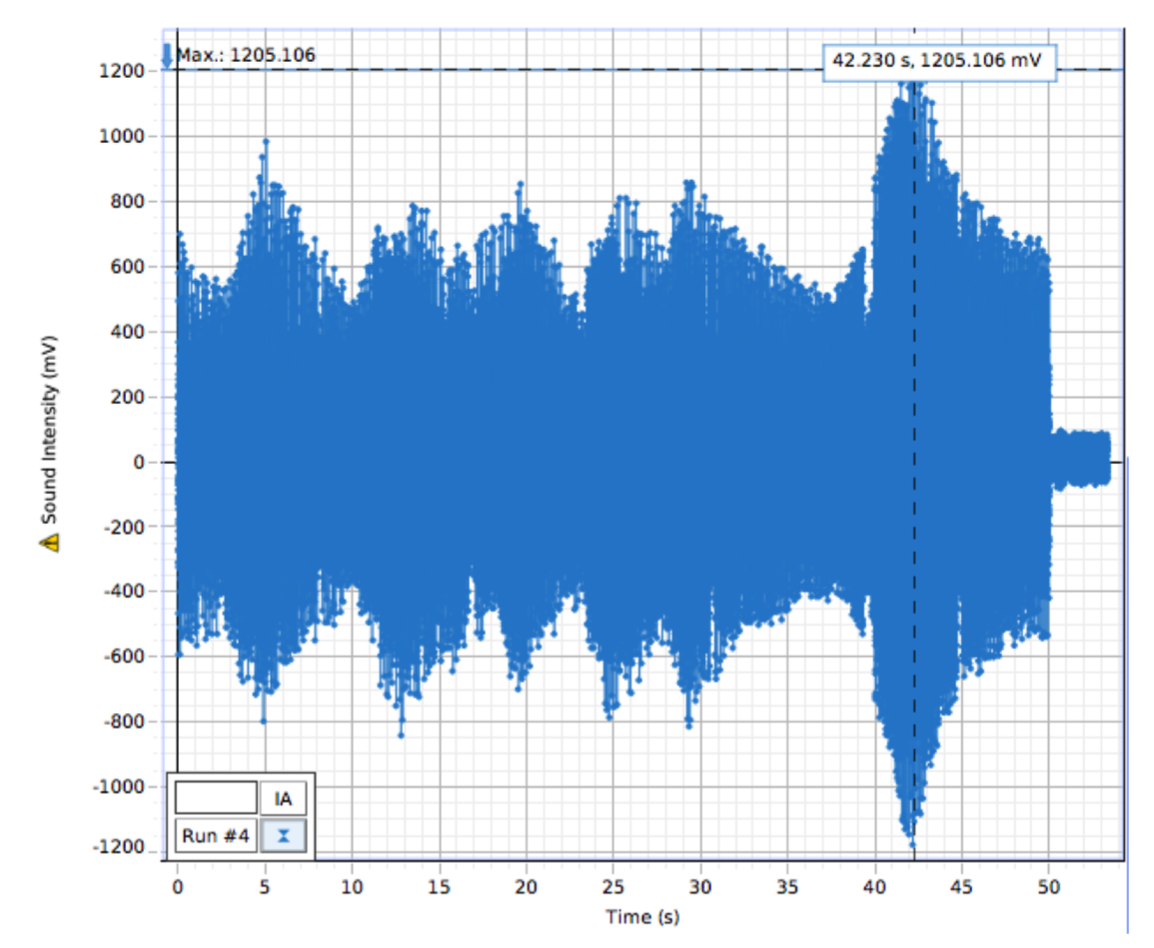
\includegraphics[width=.45\linewidth]{/home/vitowu/Documents/CourseMaterials/CourseMaterials/PHY1002-Physics_Laboratory/e7/80cm.png}
	 	}
	 	\subfigure{}{
	 		\centering
	 		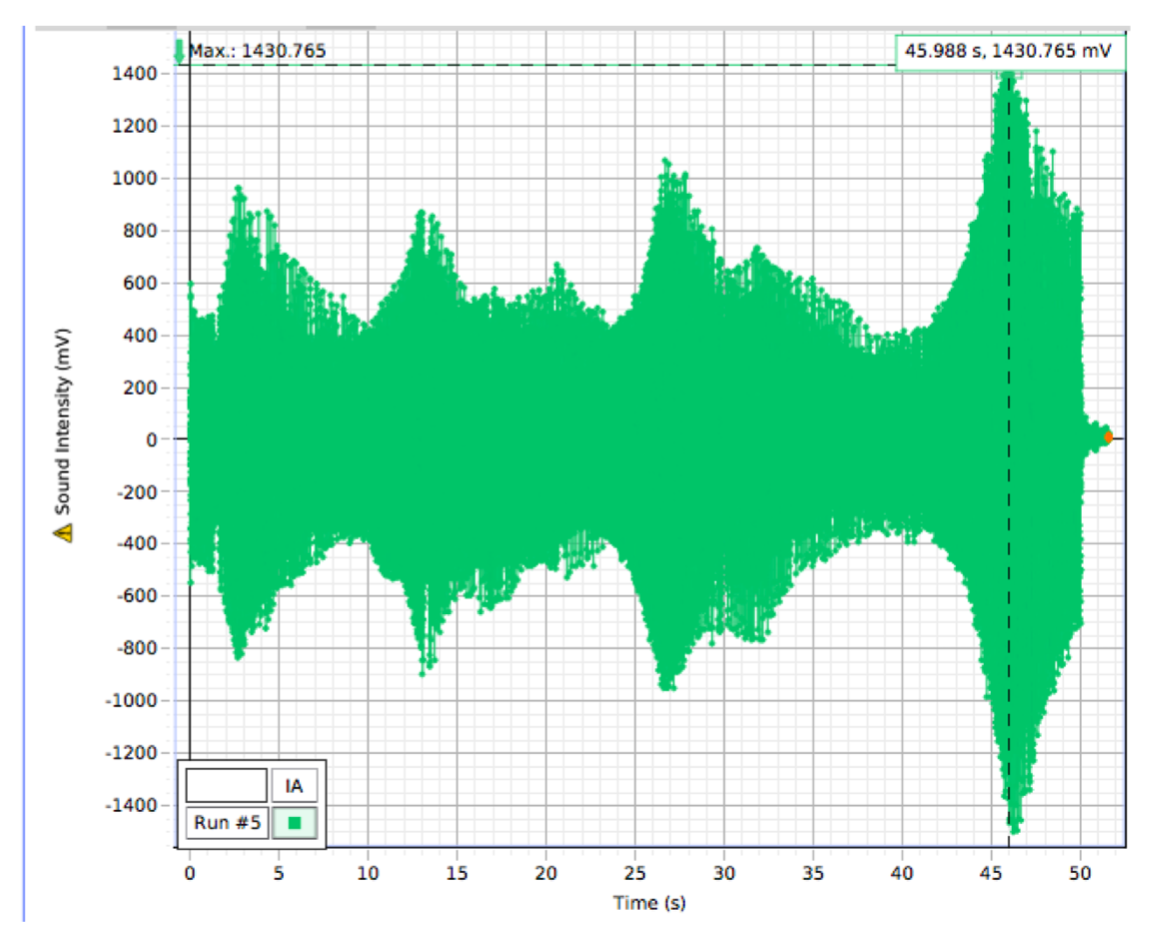
\includegraphics[width=.45\linewidth]{/home/vitowu/Documents/CourseMaterials/CourseMaterials/PHY1002-Physics_Laboratory/e7/70cm.png}
	 		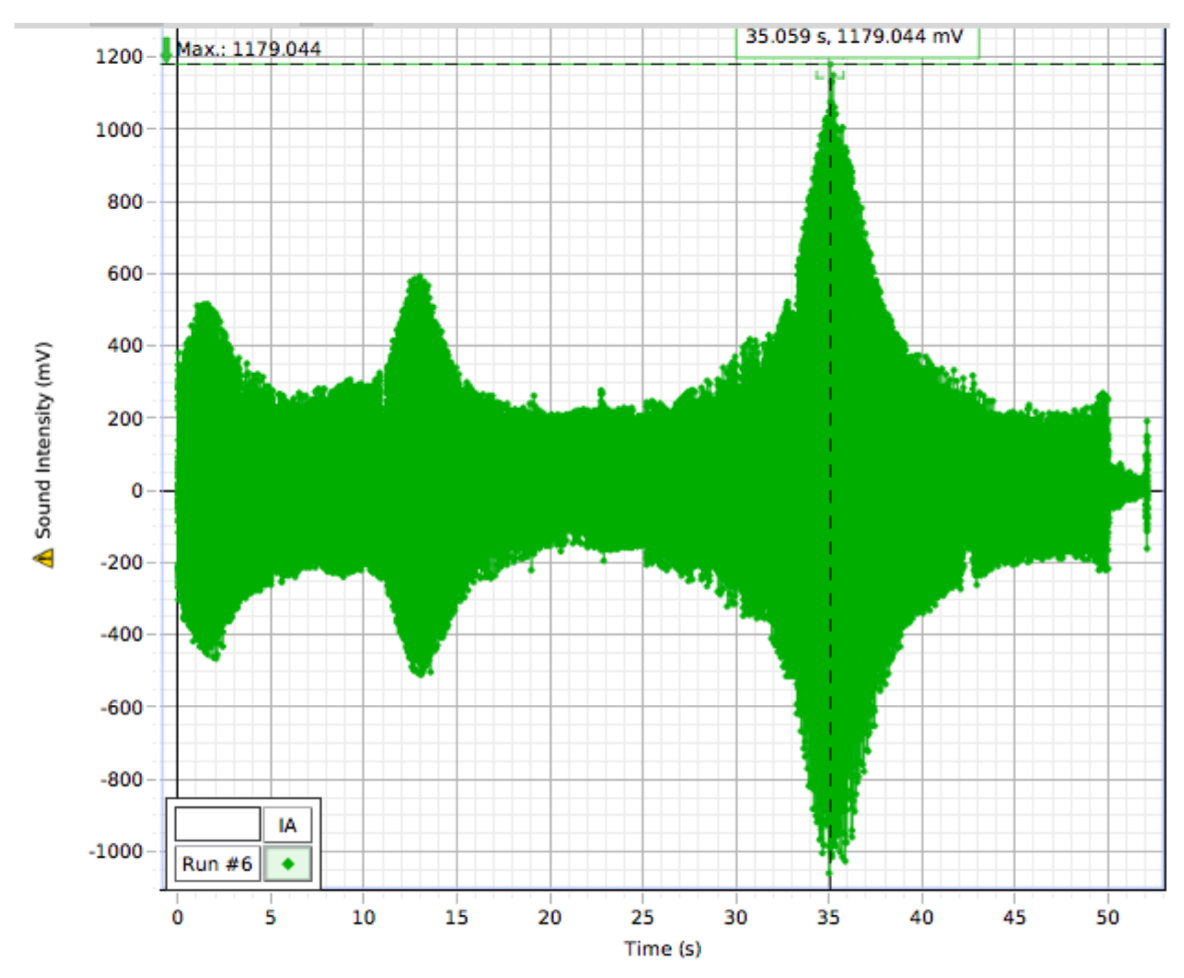
\includegraphics[width=.45\linewidth]{/home/vitowu/Documents/CourseMaterials/CourseMaterials/PHY1002-Physics_Laboratory/e7/60cm.png}
	 	}
 	\end{figure}
 	\begin{figure}[H]
 		\subfigure{}{
 			\centering
 			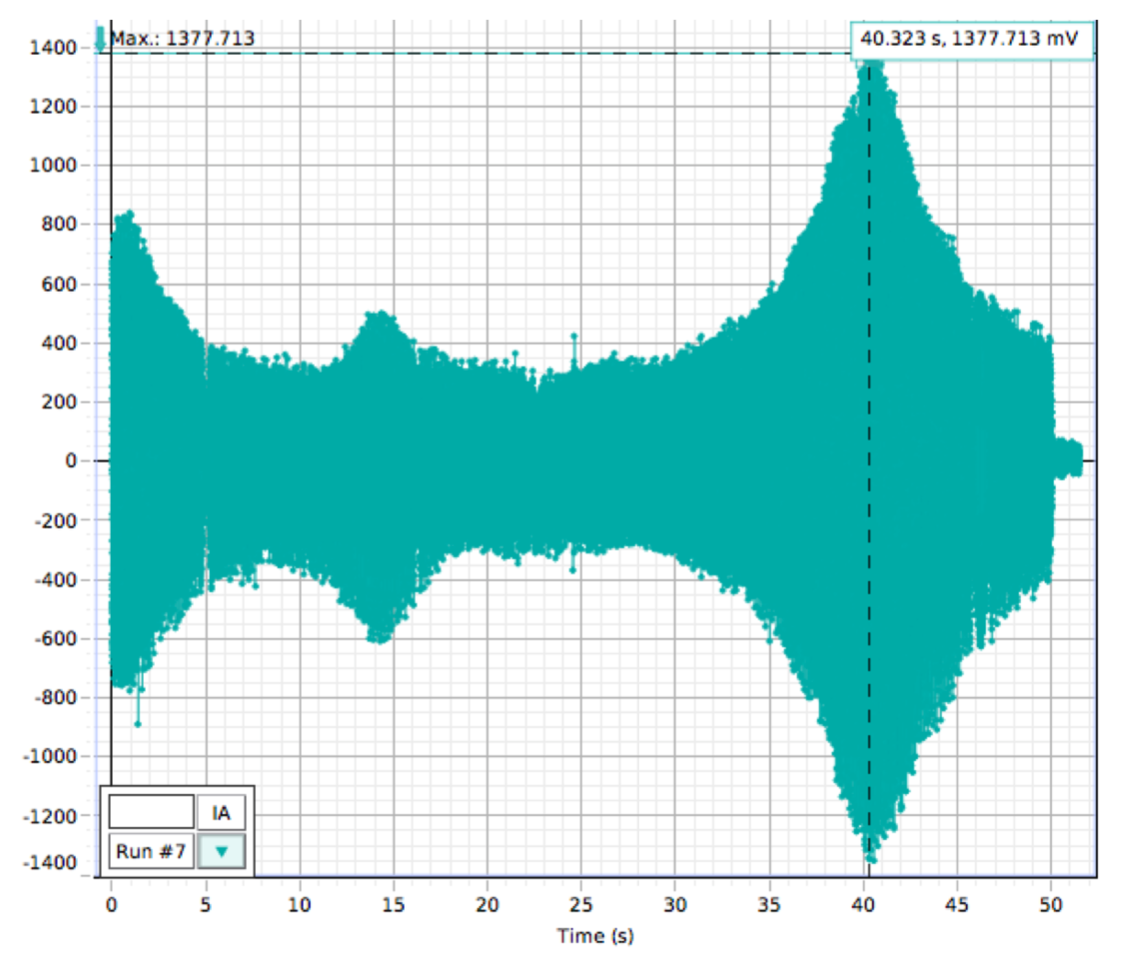
\includegraphics[width=.45\linewidth]{/home/vitowu/Documents/CourseMaterials/CourseMaterials/PHY1002-Physics_Laboratory/e7/50cm.png}
 			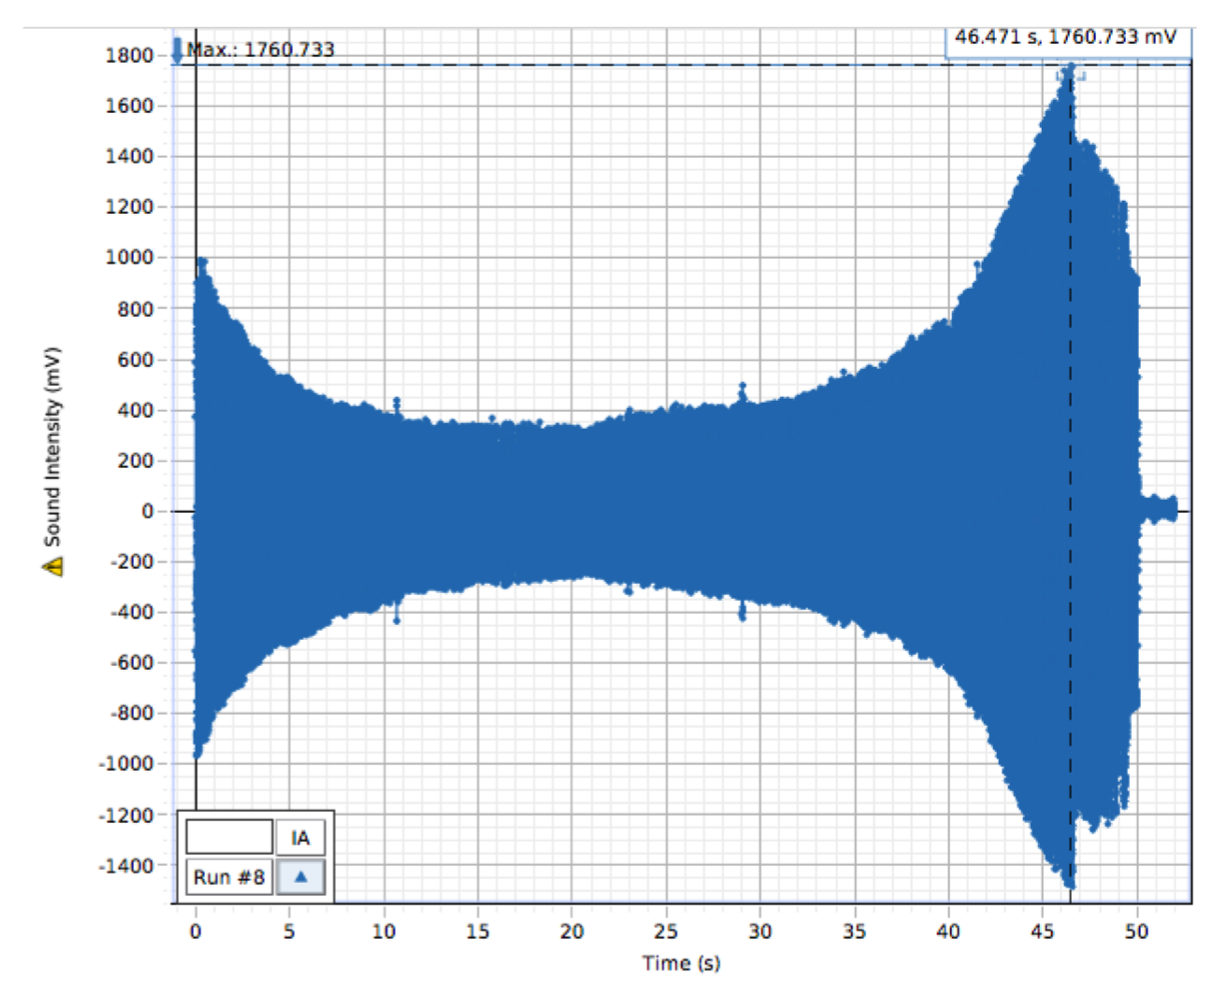
\includegraphics[width=.45\linewidth]{/home/vitowu/Documents/CourseMaterials/CourseMaterials/PHY1002-Physics_Laboratory/e7/40cm.png}
 		}
 		\caption{Experimental Data at 10 cm Intervals Down to A Length of 40 cm}
 	\end{figure}
 	To simplify the experimental results we collected and to capture the kernel of the result itself, we choose the data we want and collect them in the table as following,
 	\begin{table}[H]
 		\centering
 		\makebox[\linewidth]{
 			\begin{tabular}{|c|c|}
 				\hline
 				\hline
 				\textbf{$\L$($m$)} & \textbf{Frequency (Hz)} \\
 				\hline
 				$1.1\pm 0.0005$ & $77.103\pm 0.0005$ \\
 				\hline
 				$1.0\pm 0.0005$ & $84.127\pm 0.0005$ \\
 				\hline
 				$0.9\pm 0.0005$ & $92.487\pm 0.0005$ \\
 				\hline
 				$0.8\pm 0.0005$ & $102.230\pm 0.0005$ \\
 				\hline
 				$0.7\pm 0.0005$ & $115.988\pm 0.0005$ \\
 				\hline
 				$0.6\pm 0.0005$ & $135.059\pm 0.0005$ \\
 				\hline
 				$0.5\pm 0.0005$ & $160.323\pm 0.0005$ \\
 				\hline
 				$0.4\pm 0.0005$ & $196.471\pm 0.0005$ \\
 				\hline
 			\end{tabular}
	}
 			\caption{Fundamental Frequencies Corresponding to Different Lengths}
 	\end{table}
 	\subsubsection{Experiment 2}
 	\begin{figure}[H]
 		\centering
 		\subfigure{}{
 			\centering
 			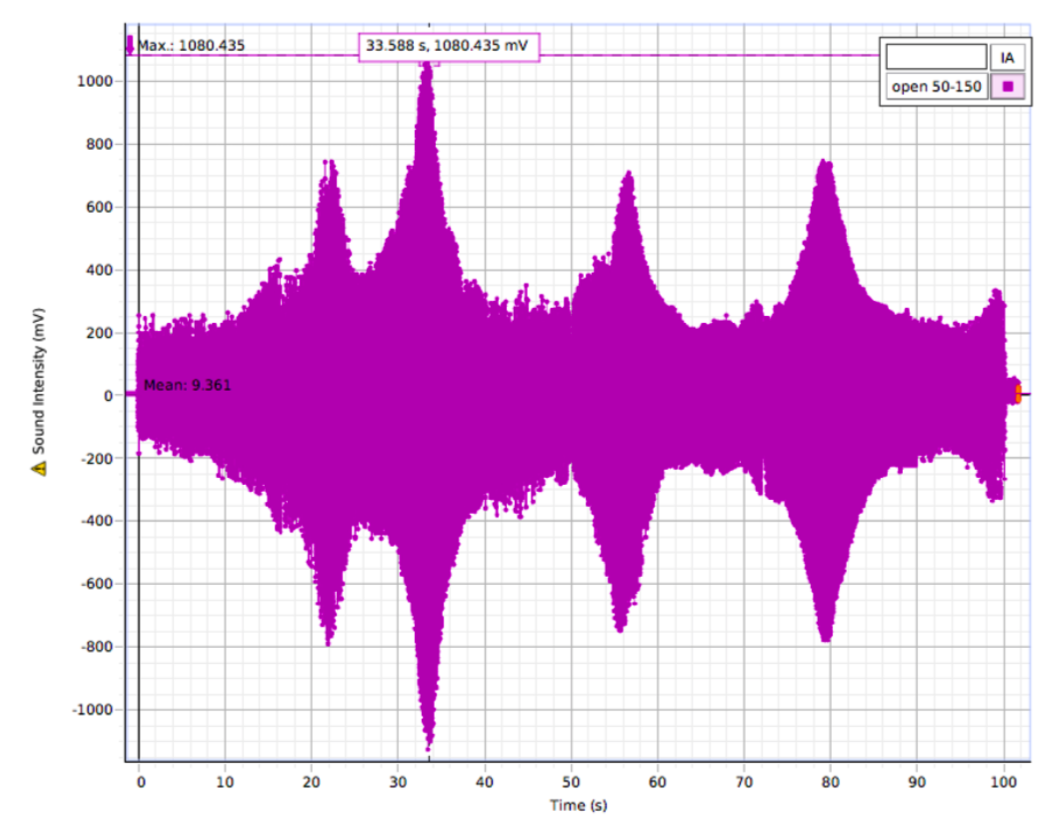
\includegraphics[width=.45\linewidth]{/home/vitowu/Documents/CourseMaterials/CourseMaterials/PHY1002-Physics_Laboratory/e7/first.png}
 			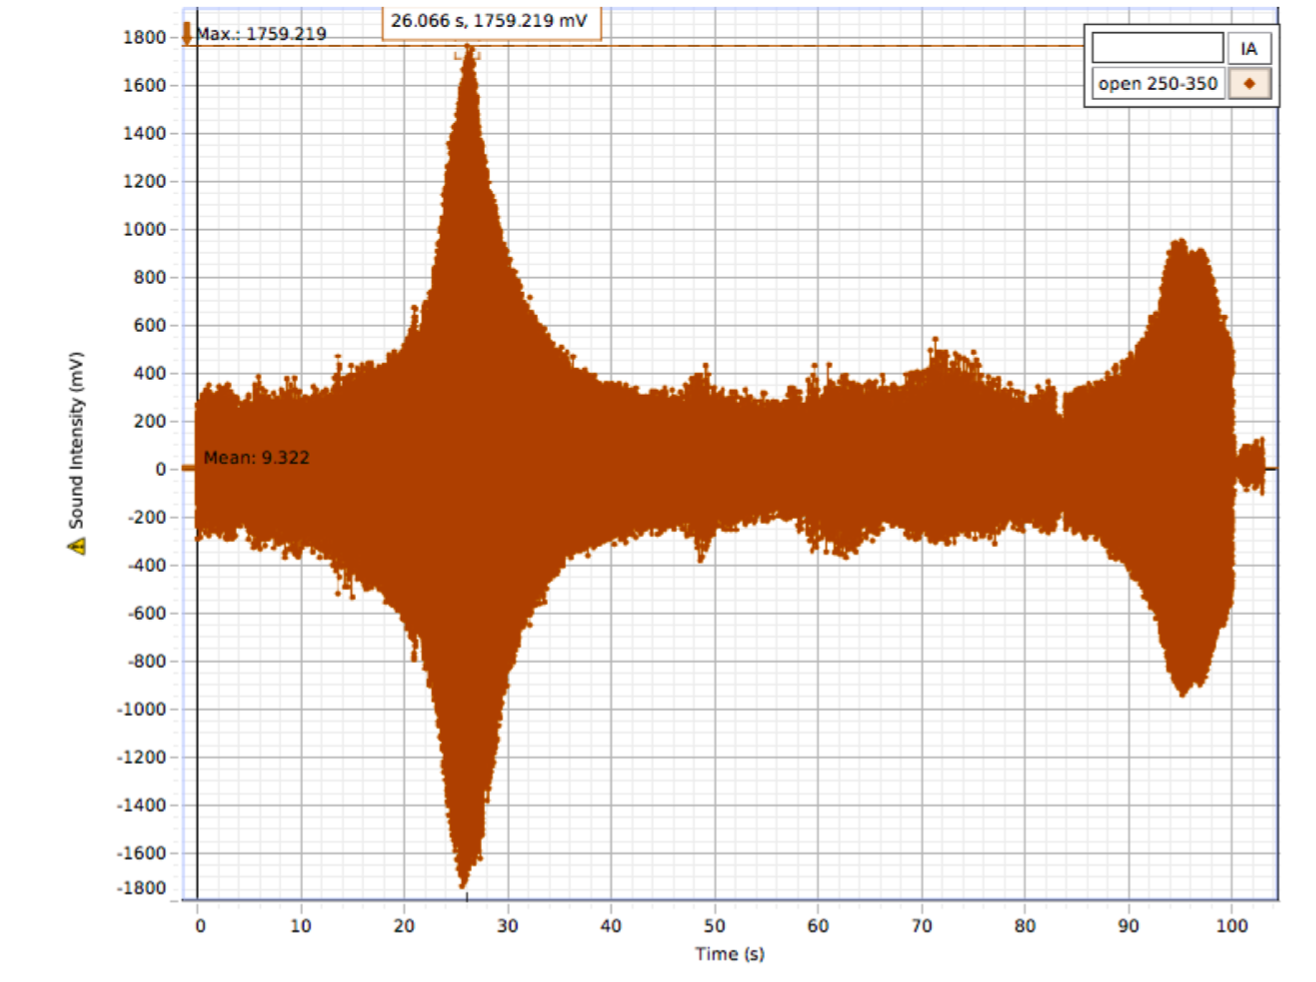
\includegraphics[width=.45\linewidth]{/home/vitowu/Documents/CourseMaterials/CourseMaterials/PHY1002-Physics_Laboratory/e7/second.png}
 		}
 	\end{figure}
 	\begin{figure}[H]
 		\subfigure{}{
 			\centering
 			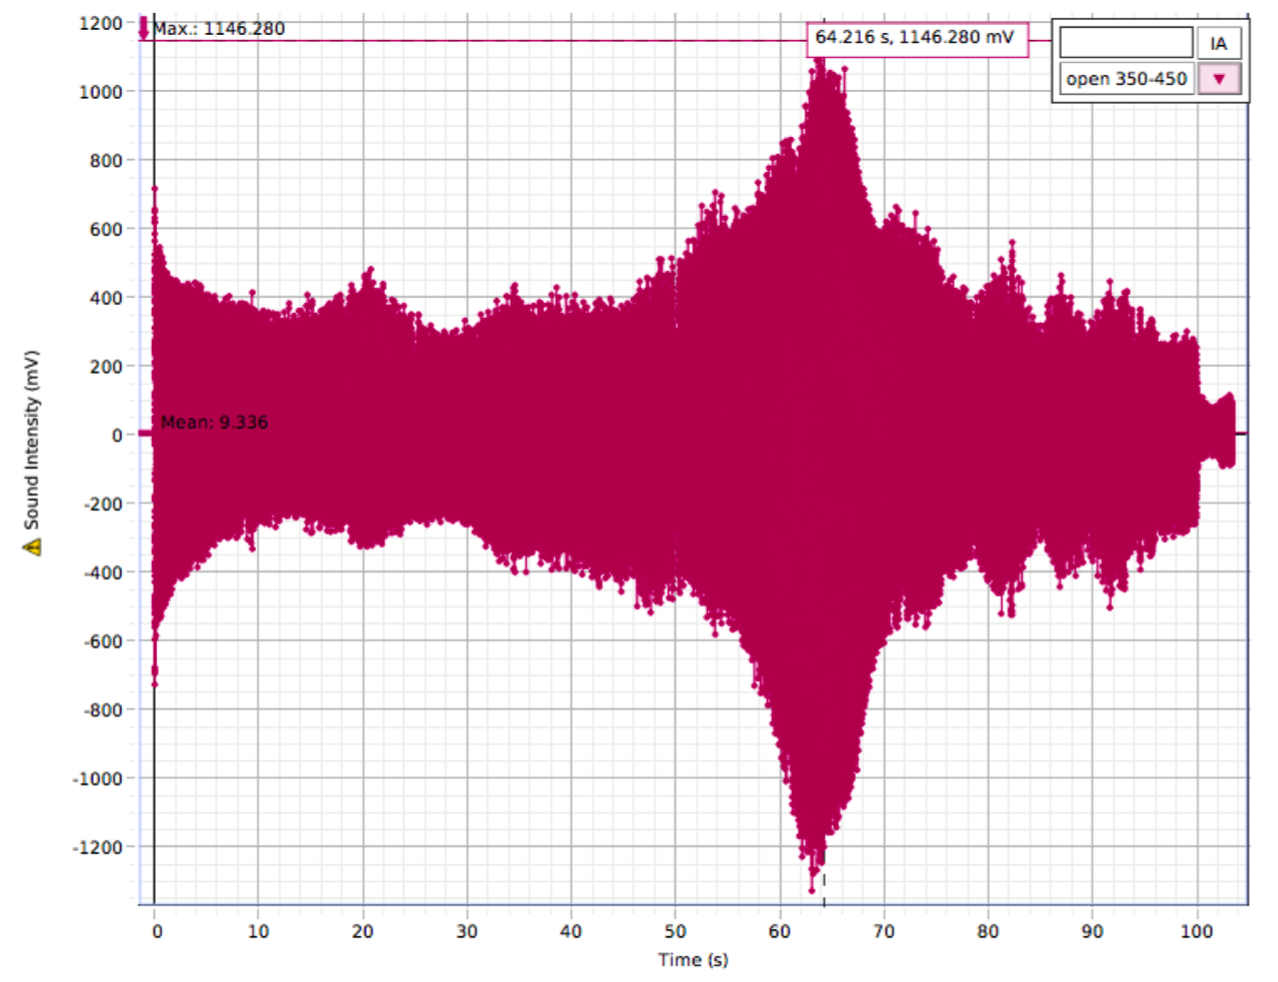
\includegraphics[width=.45\linewidth]{/home/vitowu/Documents/CourseMaterials/CourseMaterials/PHY1002-Physics_Laboratory/e7/third.png}
 			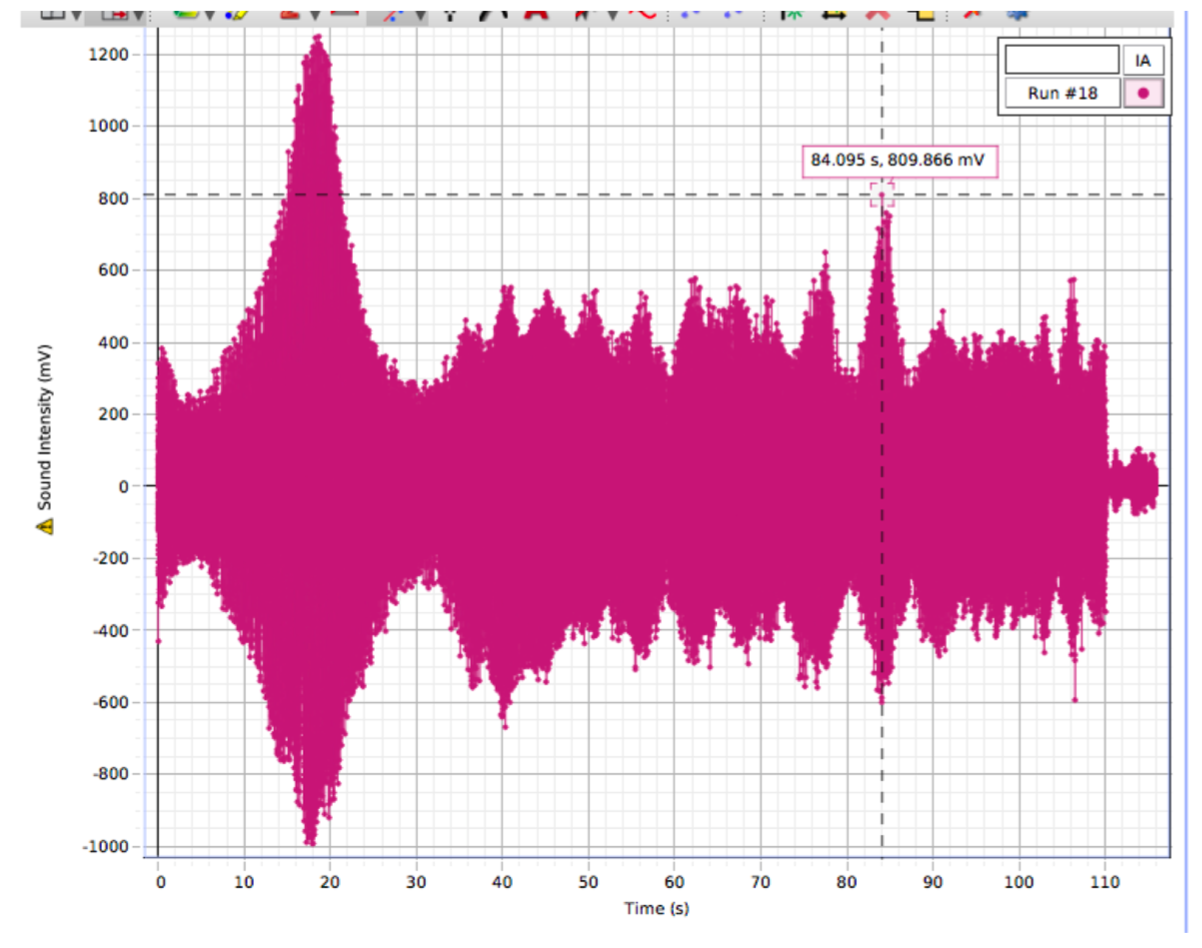
\includegraphics[width=.45\linewidth]{/home/vitowu/Documents/CourseMaterials/CourseMaterials/PHY1002-Physics_Laboratory/e7/fourth.png}
 		}
 		\caption{The First, Second, Third and Fourth Harmonics of Closed Tube}
 	\end{figure}
 	\subsubsection{Physical Data}
 	\begin{itemize}
 		\item The diameter $d = 0.08\pm 0.0005 m$
 	\end{itemize}
 	Similarly, we can collect the experimental results we used for calculation in a table as following,
 	\begin{table}[H]
 		\centering
 		\makebox[\linewidth]{
 			\begin{tabular}{|c|c|}
 				\hline
 				\hline
 				\textbf{Harmonic Type} & \textbf{Frequency (Hz)}\\ 
 				\hline
 				First Harmonic & $133.588\pm 0.0005$ \\
 				\hline
 				Second Harmonic & $276.066\pm 0.0005$ \\
 				\hline
 				Third Harmonic & $414.216\pm 0.0005$ \\
 				\hline 
 				First Harmonic (closed) & $65.905\pm 0.0005$ \\
 				\hline
 			\end{tabular}
 		}
 		\caption{Fundamental Frequencies Corresponding to Different Lengths}
 	\end{table}
 	\section{Data \& Error Analysis}
 	\subsection{Data Calculation}
 	Since that we need to plot a graph The inverse of frequency \textbf{invf} is determined only by the frequency, therefore
 	\begin{equation}
 		\delta \textbf{inv}f = \sqrt{(\delta f)^2\frac{1}{f^4}}
 	\end{equation}
 	Then in the linear regression line $y = ax + b$, a and b is obtained by the equation
 	\begin{equation}
 		\arg_{min}\frac{1}{n}\sum_{i = 1}^{n}(L_i-ax_i-b)^2
 	\end{equation}
 	\begin{equation}
 		\delta L = \sqrt{\frac{1}{n-2}\sum_{i=1}^{n}(L_i-ax_i-b)^2}
 	\end{equation}
 	And for coefficient a and b,
 	\begin{equation}
 		\delta a = \delta L\sqrt{\frac{n}{n\sum_{i=1}^{n}x_i^2 - (\sum_{i=1}^{n}x_i)^2}}
 	\end{equation}
 	\begin{equation}
 		\delta b = \delta L\sqrt{\frac{\sum_{i=1}^{n}x_i^2}{n\sum_{i=1}^{n}x_i^2 - (\sum_{i=1}^{n}x_i)^2}}
 	\end{equation}
 	The first approach to obtain the speed of sound in air $ v $ is calculated from the regression line. Since the slope of the regression curve $a = \frac{1}{4v}$,
 	\begin{equation}
 		\delta v_1 = \sqrt{(\delta a)^2 (\frac{-1}{4a^2})^2}
 	\end{equation}
 	The second approach to obtain the speed of sound is using equation 7,
 	\begin{equation}
 		\delta v_2 = \sqrt{(\delta f)^2((2n-1)\frac{-v}{4f^2}^2)}
 	\end{equation}
 	The third approach to obtain the speed of sound is using equation 9,
 	\begin{equation}
 		\delta v = \sqrt{(\delta f)^2(n\frac{-vf}{2f^2})^2}
 	\end{equation}
 	The calculated harmonic frequencies f depend on the diameter and length of tube, hence for closed tube,
 	\begin{equation}
 		\delta f = \sqrt{(\delta d)^2(\frac{-0.3}{4(l+0.3d)^2})^2+(\delta l^2)(\frac{-1}{4(l+0.3d)^2})^2}
 	\end{equation}
 	For the open cube,
 	\begin{equation}
 		\delta f = \sqrt{(\delta d)^2(\frac{-0.6}{2(l+0.6d)^2})^2 + (\delta l)^2(\frac{-1}{2(l+0.6d)^2})^2}
 	\end{equation}
 	From the experimental results in Experiment 1, we can plot a linear fit graph on L versus invf.
 	\begin{figure}[H]
 		\subfigure{}{
 			\centering
 			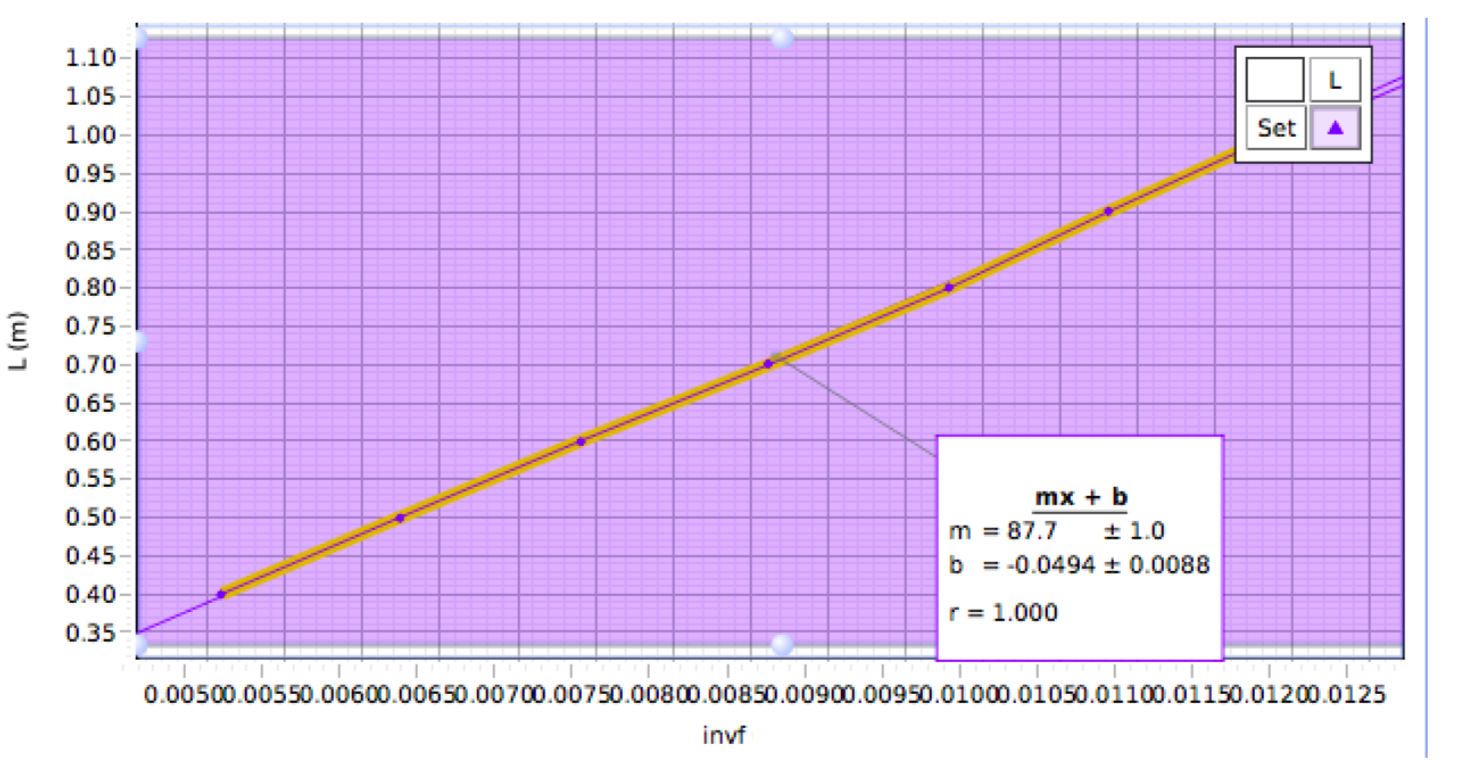
\includegraphics[width=.9\linewidth]{/home/vitowu/Documents/CourseMaterials/CourseMaterials/PHY1002-Physics_Laboratory/e7/LinearFit.png}
 		}
 	\end{figure}
 	Using the experimental results and the theoretical equations, we can obtain that $L = (87.7\pm1.0)x-(0.0494\pm0.0088)$, and speed of sound $v = 350.8\pm0.005 m/s$.
 	\begin{table}[H]
 		\centering
 		\makebox[\linewidth]{
 			\begin{tabular}{|c|c|c|}
 				\hline
 				\hline
 				L(m) & $f_{theory}$(Hz) & Difference \\
 				\hline
 				$ 1.1\pm0.0005 $ & $ 79.727\pm0.002 $ & $ -3.29\% $ \\
 				\hline
 				$ 1.0\pm0.0005 $ & $ 87.700\pm0.002 $ & $ -4.07\% $ \\
 				\hline
 				$ 0.9\pm0.0005 $ & $ 97.444\pm0.002 $ & $ -5.09\% $ \\
 				\hline
 				$ 0.8\pm0.0005 $ & $ 109.625\pm0.003 $ & $ -6.75\% $ \\
 				\hline
 				$ 0.7\pm0.0005 $ & $ 125.286\pm0.003 $ & $ -7.42\% $ \\
 				\hline
 				$ 0.6\pm0.0005 $ & $ 146.167\pm0.003 $ & $ -7.60\% $ \\
 				\hline
 				$ 0.5\pm0.0005 $ & $ 175.400\pm0.003 $ & $ -8.60\% $ \\
 				\hline
 				$ 0.4\pm0.0005 $ & $ 219.25\pm0.003 $ & $ -10.39\% $ \\
 				\hline
 			\end{tabular}
 		}
 		\caption{Theoretical Fundamental Frequencies of Closed Tube in Experiment 1}
 	\end{table}
	\begin{table}[H]
	 	\centering
	 	\makebox[\linewidth]{
	 		\begin{tabular}{|c|c|c|}
	 			\hline
	 			\hline
	 			Harmonic Type & $ f_{theory} $(Hz) & Difference \\
	 			\hline
	 			First Harmonic & $ 141.452\pm0.004 $ & $ 5.89\% $ \\
	 			\hline
	 			Second Harmonic & $ 282.903\pm0.004 $ & $ 2.48\% $ \\
	 			\hline
	 			Third Harmonic & $ 424.355\pm0.007 $ & $ 2.45\% $ \\
	 			\hline
	 			First Harmonic(closed) & $ 70.726\pm0.002 $ & $ 7.32\% $ \\
	 			\hline
	 		\end{tabular}
	 	}
	 	\caption{Theoretical Fundamental Frequencies of Closed Tube in Experiment 2}
	\end{table}
	\subsection{Data Analysis}
	As the data above show that the difference between experimental results and theoretical results is acceptable, it is reasonable to conclude that the experiment supports and verifies the theories.\par 
	However, from the data we notice a phenomenon that the differences of theoretical results and the experimental results increases as the length of the air column increases, and we guess that there exist a systematical error which relates to the length of the air column. We will try to answer the questions we found in the experiment in the next chapter.
	\section{Questions}
	\subsection{Experiment 1}
	\textbf{1.} On your graph of L vs. invf, why isn't the y-intercept zero? \par 
	Answer: As described in the theory part, the exact effective air column is slightly longer than the air column in the tube, which means the anti node is actually outside the tube, and therefore the y-intercept isn't zero. \par
	\textbf{2.} Is the intercept negative? \par
	Answer: As shown in the result, it is $ 0.0494\pm0.0088 $ \par
	\textbf{3.} How does this value for the extra end-effect length compare with the y-intercept of your graph?\par 
	Answer: The error is significant so there exists systematic error. From what shown in the table 3 and table 4, the end-effect will increase as the length of the tube increase.
	\subsection{Experiment 2}
	\textbf{1.} Why is the frequency of the fundamental higher for the open tube than it was for the closed tube? \par 
	Answer: Inferred from the theoretical equations, the denominator of Experiment 1 is 4, while the denominator of Experiment 2 is 2. When the velocity of sound and the length of the tube does not change, the fundamental frequency of Experiment 2 will higher than the Experiment 1. \par
	\textbf{2.} How does the actual tube length compare to the effective length?\par 
	Answer: The measured tube length is $ 1.2000\pm0.005 $m, and the calculated actual tube length $ L_{actual} = L_{measured}+0.6d = 1.28000\pm0.0014$m. Using the equation 1 we calculate the effective length $ L_{effective} = 1.190\pm0.0006 $m, which lies in the range of measured length.\par
	\textbf{3.} When the frequency was returned to the fundamental, and the end of the tube was closed, was it still in resonance?\par
	Answer: No, according to the theoretical equation 1 and 2, we can find that no integer n can satisfy the fundamental frequency of open tube, which means no resonance occurs.\par
	\textbf{4.} What should the ratio of the open-tube frequency to the closed-tube frequency be? Why?\par 
	Answer: The ratio of of the first, second, third harmonic frequency of the open tube to the first frequency of closed tube should be 2, 4, 6 respectively. According to the theory, the first, second, third harmonic frequency of open tube is $ \frac{v}{2L} $, $ \frac{v}{L} $, $ \frac{3v}{2L} $, and the first harmonic frequency of open tube is $ \frac{v}{4L} $.
	\section{Conclusion}
	In the experiment, we explore the fundamental frequencies with different air column length and the resonance frequencies under difference resonance modes with fixed air column length. We found that our results supports the prediction of theory with a small difference. We tried to analysis the error and give our illustration to the questions we found in the experiment.
	
\end{document}
